\chapter{多时间尺度快慢系统慢流形的隐式近似方法}\label{chapter:two}
\fancyhead[CO]{\leftmark~~多时间尺度快慢系统慢流形的隐式近似方法}
\section{引言}

\begin{figure}[htbp]
\setlength{\belowcaptionskip}{-15.0pt}
  \centering
 \subfigure[系统lorenz数值结果]{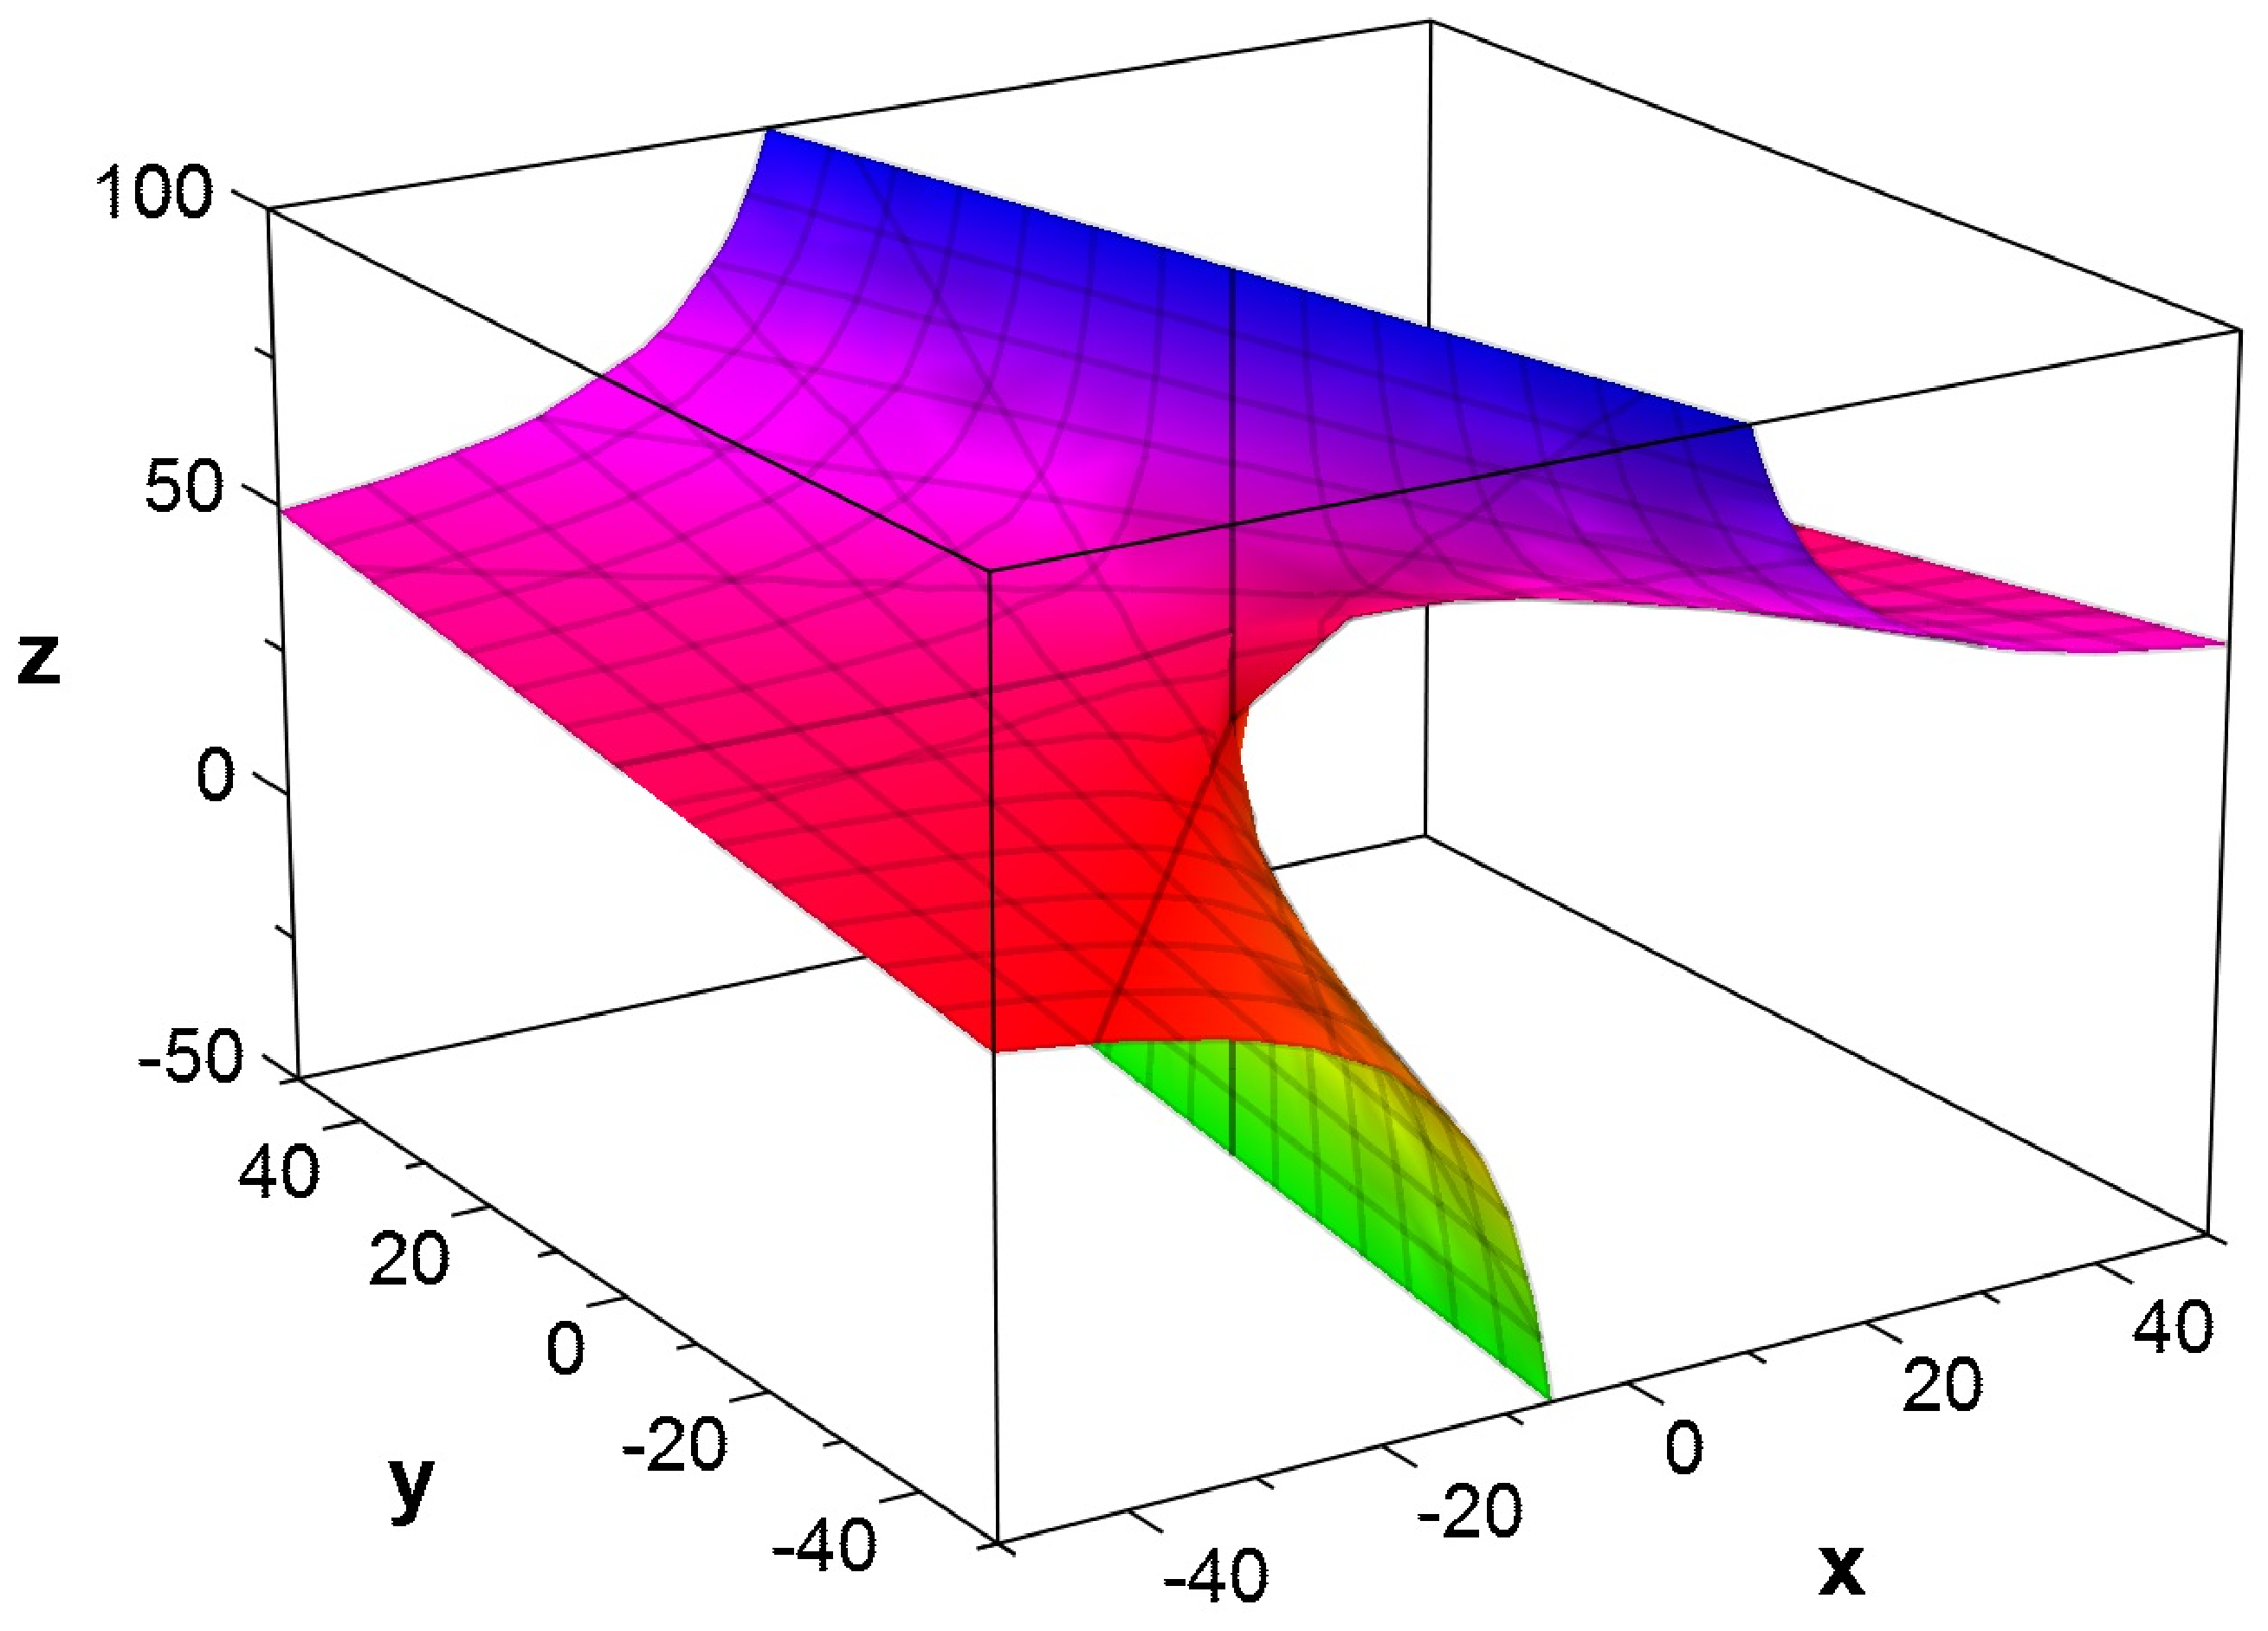
\includegraphics[width=5cm,height=5cm]{fig/sec2_lorenz_manifold2.eps}}
 \subfigure[系统van der pol数值结果]{\includegraphics[width=5cm,height=5cm]{fig/sec2_vandp_2.eps}}
 \subfigure[系统BZ,$z=0$平面上数值结果] {\includegraphics[width=5cm,height=5cm]{fig/sec2_BZ_ser3.eps}}
  \caption{三类不同系统数值结果.}\label{fig:three_type}
\end{figure}

\newpage
\mbox{}
\newpage




























